\documentclass[12pt]{beamer}
\usetheme{Warsaw}
\usepackage[utf8]{inputenc}
\usepackage[english]{babel}
\usepackage{amsmath}
\usepackage{stmaryrd}
\usepackage{amsfonts}
\usepackage{amssymb}
\usepackage{graphicx}
\usepackage{xcolor}
\usepackage[backend=bibtex, style=authoryear, maxcitenames=2]{biblatex}
\addbibresource{../../Thesis/references.bib} 
\renewcommand*{\bibfont}{\footnotesize}
\usepackage{url}
\definecolor{lila}{RGB}{128,0,128}

\newcommand{\myCite}[1]{{\scriptsize\parencite{#1}}}

\setbeamertemplate{navigation symbols}{}
\setbeamertemplate{footline}{%
	\raisebox{5pt}{%
		\makebox[\paperwidth]{%
			\hfill\makebox[10pt]{%
				\textcolor{gray}{\footnotesize\insertframenumber}
			}
		}
	}
}

\definecolor{regal}{RGB}{81,0,0}
\usepackage{array}
\usepackage{colortbl}
\makeatletter
\newcommand{\thickhline}{%
    \noalign {\ifnum 0=`}\fi \color{regal}\hrule height 4pt
    \futurelet \reserved@a \@xhline
}
\newcolumntype{"}{@{\color{regal}\hskip\tabcolsep\vrule width 8pt\hskip\tabcolsep}}
\makeatother

% listings
\usepackage[TS1,T1]{fontenc}
\usepackage{newunicodechar}
\newcommand*\longs{{\fontencoding{TS1}\selectfont s}}
\newunicodechar{ſ}{\longs}
\usepackage{listings}
\definecolor{mygreen}{rgb}{0,0.6,0}
\definecolor{mygray}{rgb}{0.5,0.5,0.5}
\definecolor{mymauve}{rgb}{0.58,0,0.82}
\lstset{
	captionpos=b,
	frame=single,
	breaklines=true,
	breakatwhitespace=true,
	literate=%
		{Ö}{{\"O}}1
		{Ä}{{\"A}}1
		{Ü}{{\"U}}1
		{ß}{{\ss}}1
		{ü}{{\"u}}1
		{ä}{{\"a}}1
		{ö}{{\"o}}1
		{~}{{\textasciitilde}}1,
	tabsize=4,
	aboveskip=4pt,
	belowskip=6pt,
	backgroundcolor=\color{white},   % choose the background color
	basicstyle=\footnotesize,        % size of fonts used for the code
	breaklines=true,                 % automatic line breaking only at whitespace
	captionpos=b,                    % sets the caption-position to bottom
	commentstyle=\color{mygreen},    % comment style
	escapeinside={\%*}{*)},          % if you want to add LaTeX within your code
	keywordstyle=\color{blue},       % keyword style
	stringstyle=\color{mymauve},     % string literal style
}
\definecolor{maroon}{rgb}{0.5,0,0}
\definecolor{darkgreen}{rgb}{0,0.5,0}
\lstdefinelanguage{XML}
{
	basicstyle=\ttfamily\tiny,
	morestring=[s]{"}{"},
	morecomment=[s]{?}{?},
	morecomment=[s]{!--}{--},
	commentstyle=\color{darkgreen},
	moredelim=[s][\color{black}]{>}{<},
	moredelim=[s][\color{red}]{\ }{=},
	stringstyle=\color{blue},
	identifierstyle=\color{maroon}
}

%\setbeamercovered{transparent} 
%\logo{}  
%\subject{} 
\begin{document} 
		
\begin{frame}[plain,noframenumbering]
	\begin{minipage}{0.1\textwidth}
		\hspace{-0.5cm}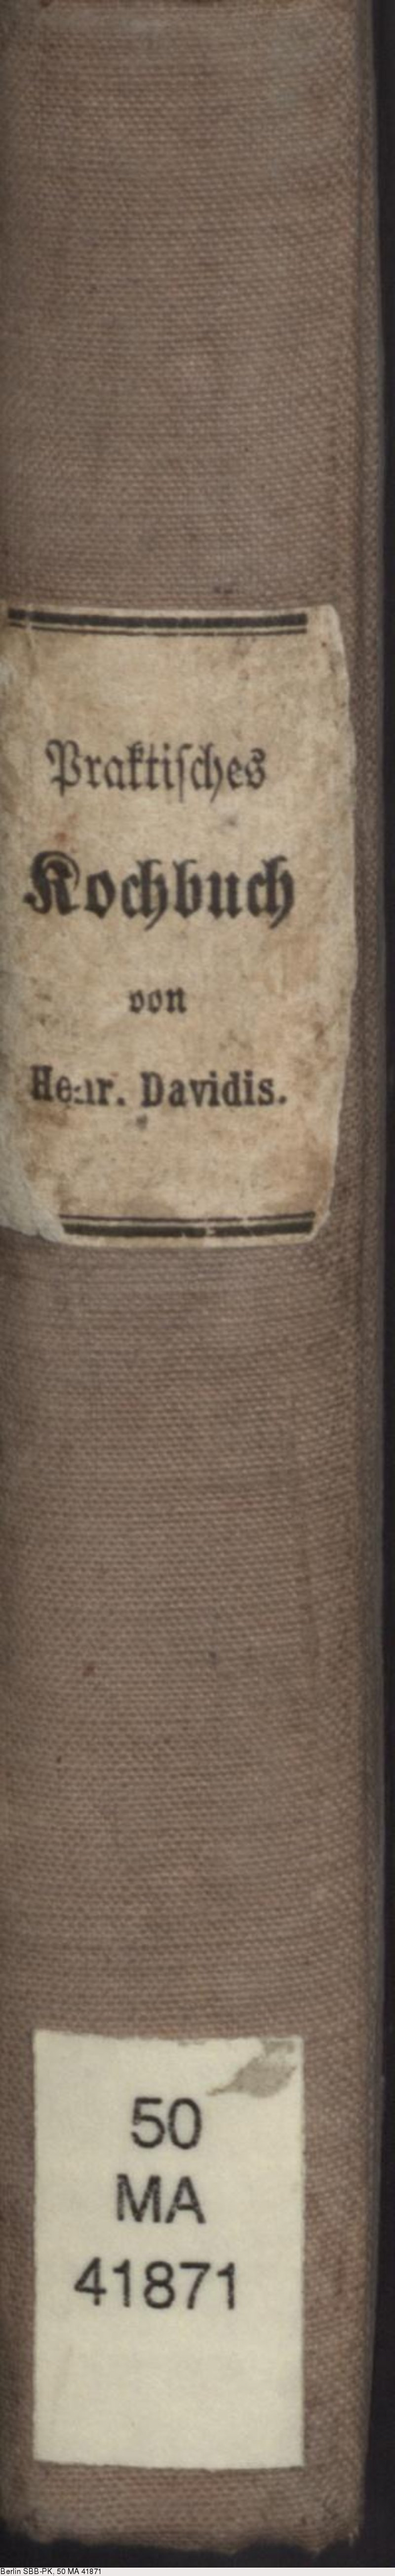
\includegraphics[scale=0.049]{../Buchruecken}
	\end{minipage}
	\begin{minipage}{0.6\textwidth}
		\begin{center}
			\vspace{-1.5cm}
			\Large{Extracting recipe ingredients \\ from cookbooks} \\
			\vspace{0.5cm}
			\large{Ritter und Fabelwesen} \\
			\small{von \\ \vspace{-0.1cm} Torsten Knauf}
		\end{center}
	\end{minipage}
	\begin{minipage}{0.25\textwidth}
		\arrayrulecolor{red}
		\small
		\begin{tabular}{"l}
			Der Beginn einer \\ Master-Arbeit \\
			\thickhline
			\color{white} \\
			Irrlichter \\
			\thickhline 
			Heraus aus \\
			dem Sumpf \\
			\thickhline 
			\color{white} - \\
			\color{white} - \\
			\thickhline 
			\color{white} - \\
			\color{white} - \\
			\thickhline 
			\color{white} - \\
			\color{white} - \\
			\thickhline 
			\color{white} - \\
			\color{white} - 
		\end{tabular}
	\end{minipage}
\end{frame}


\begin{frame}{Contents}
	\begin{enumerate}
		\item Introduction
		\item Making a cookbook machine readable
		\item Related Work
		\item CRF-based extraction
		\item Dictionary- and Rule-based extraction
		\item Discussion
		\item Summary
	\end{enumerate}
\end{frame}	

\begin{frame}{2. Making a cookbook machine readable}
	\begin{enumerate}
		\item Digitalisation
		\item CueML ontology
		\item Need for automation
	\end{enumerate}
\end{frame}

\begin{frame}{3. Related Work}
	\begin{enumerate}
		\item Skip The Pizza
		\item Extracting Structured Data From Recipes Using Conditional Random
		Fields
		\begin{enumerate}
			\item CRF
			\item Implementation of NYT
		\end{enumerate}
		\item Domain Specific Information Extraction for Semantic Annotation
		\item Data-driven Knowledge Extraction for the Food Domain
		\item Lessons for this work
	\end{enumerate}
\end{frame}

\begin{frame}{4. CRF-based extraction}
	\begin{enumerate}
		\item CRF prototype
		\item Evaluation
	\end{enumerate}
\end{frame}

\begin{frame}{5. Dictionary- and Rule-based extraction}
	\vspace{-0.3cm}\begin{center}
		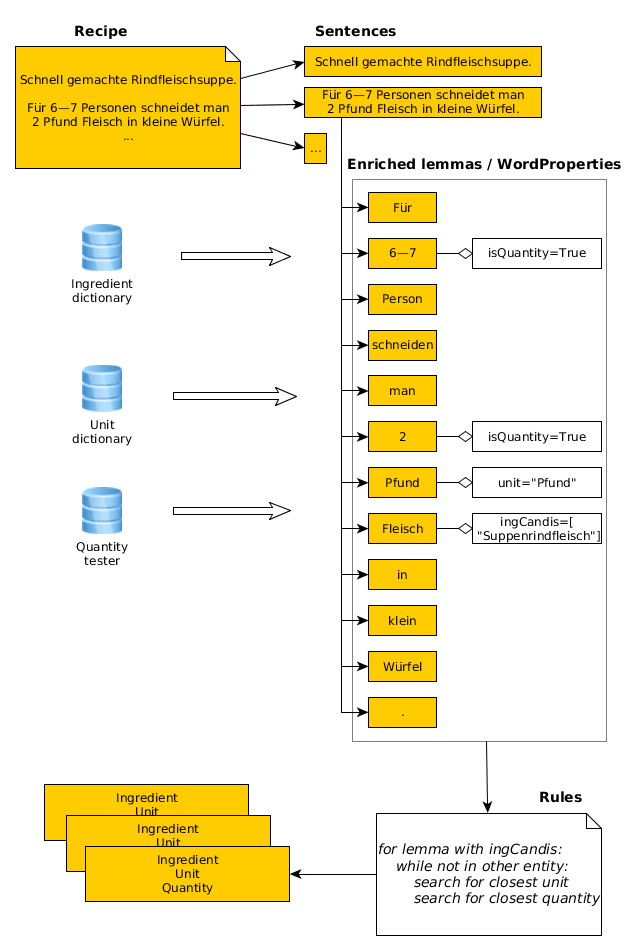
\includegraphics[width=1\linewidth, height=\textheight,keepaspectratio]{../../Images/dictBasedExtraction}
	\end{center}
\end{frame}

\begin{frame}[fragile]{5. Dictionary- and Rule-based extraction}
	\begin{minipage}{0.4\textwidth}
		\begin{lstlisting}[language=XML, caption={Auszug aus cue:listIngredients}]
<cue:ingredient xml:id="Midder" BLSref="V582100">
	<cue:prefBasicForm>
		Midder
	</cue:prefBasicForm>
	<cue:altBasicForm>
		Kalbsmidder
	</cue:altBasicForm>
	<cue:altBasicForm>
		Bries
	</cue:altBasicForm>
	<cue:altBasicForm>
		Kalbsmilch
	</cue:altBasicForm>
	<cue:note>
		"Kalbsmidder ist auch
		unter dem Synonym [...]"
		(http://www.[...])
	</cue:note>
</cue:ingredient>
<cue:ingredient xml:id="Rindkochfleisch" BLSref="U180100">
	<cue:prefBasicForm>
		Rindfleisch
	</cue:prefBasicForm>
<cue:ingredient xml:id="Hammelfleisch" BLSref="Y400003">
	<cue:prefBasicForm>
		Hammelfleisch
	</cue:prefBasicForm>
</cue:ingredient>
		\end{lstlisting}
	\end{minipage}
	\hspace*{0.2cm}\begin{minipage}{0.57\textwidth}
		\vspace{-1cm}\begin{center}Ingredient dictionary\end{center}\vspace{-0.5cm}
		\begin{lstlisting}
{
	Midder        : V582100
	Kalbsmidder   : V582100
	[...]
	Rindfleisch   : U180100
	Hammelfleisch : Y400003
	[...]
	Fleisch       : [U180100,
	                 Y400003,
	                 ...
	                ]
}
		\end{lstlisting}
	\end{minipage}
\end{frame}

\begin{frame}{5. Dictionary- and Rule-based extraction}
	\begin{center}
		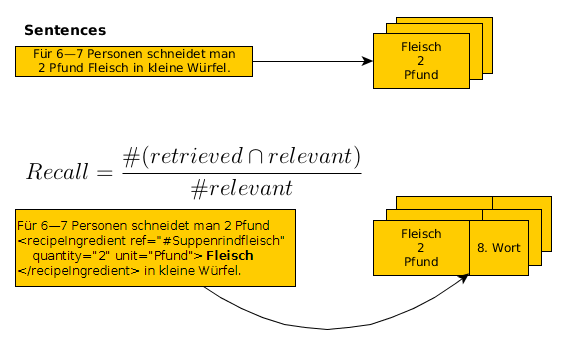
\includegraphics[width=1\linewidth, height=\textheight,keepaspectratio]{../../Images/recall}
	\end{center}
\end{frame}

\begin{frame}{5. Dictionary- and Rule-based extraction}
	\begin{center}
		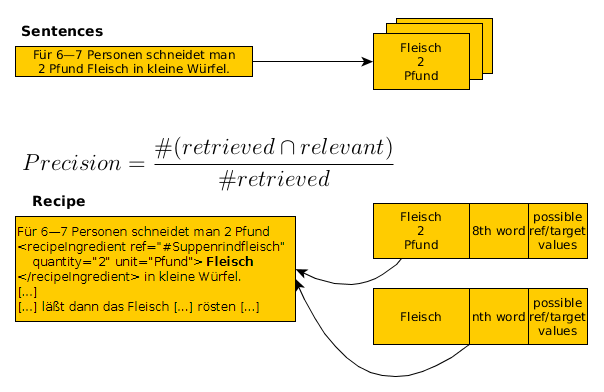
\includegraphics[width=1\linewidth, height=1\textheight, keepaspectratio]{../../Images/precision}
	\end{center}
\end{frame}

\begin{frame}{5. Dictionary- and Rule-based extraction}
	\textbf{Evaluation with recipes B-1 to B-50:}\\
	\hspace{1cm}(Only considering ingredients)\\
	\begin{itemize}
		\item Recall: 0.807 (394/488)
		\item Precision: 0.833 (434/521)
		\item Time: 144.7 seconds
		\item Flaws:
		\begin{itemize}
			\item Lemmatization (\textit{Saucissen} $\not\Rightarrow$ \textit{Saucisse})
			\item Is \textit{Brühe} an ingredient?
			\item Ingredients within title not tagged
		\end{itemize}
	\end{itemize}
\end{frame}

\begin{frame}{5. Dictionary- and Rule-based extraction}
	\begin{enumerate}
		\item Dictionary- and Rule-based prototype
		\begin{enumerate}
			\item Conceptual idea
			\item Evaluation
		\end{enumerate}
		\item Refinement of prototype
		\begin{enumerate}
			\item Illustrative enhanced rules
			\item Evaluation
		\end{enumerate}
		\item GermaNet
	\end{enumerate}
\end{frame}

\begin{frame}{6. Discussion}
	\begin{enumerate}
		\item Usefulness of automatic extraction of ingredients
		\item Quality of cueML and the obtained data
		\item The development process
		\item Knowledge is power
	\end{enumerate}
\end{frame}

\begin{frame}{(8.) Ich bin Realist}
	\begin{minipage}{0.35\textwidth}
		\vspace*{0.7cm}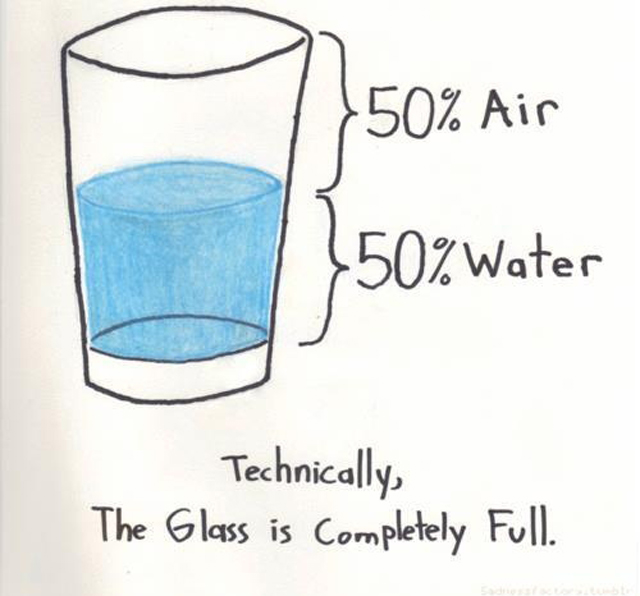
\includegraphics[width=1\linewidth]{Images/Spoken-like-a-true-realist} \\
		
		\vspace*{0.2cm}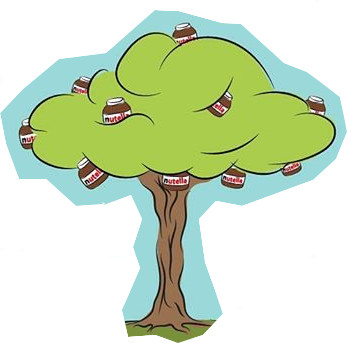
\includegraphics[width=0.9\linewidth]{Images/Nutellabaum}
	\end{minipage}
	\begin{minipage}{0.6\textwidth}
		\textbf{Ich glaube, ich kann:}
		\begin{itemize}
			\item Eine makellose Zutatenliste für jedes Rezept automatisch extrahieren
			\item Alle Informationen aus dem Buch extrahieren
			\item Eine wunderschöne Webseite zum Kochbuch erstellen und mit Inhalt füllen

			\vspace*{0.6cm}			
			\item Einen Nutellabaum pflanzen
		\end{itemize}
		
	\vspace{0.3cm}\hspace{3.5cm}\textcolor{blue}{\footnotesize{*XML-Tagger}}
	\end{minipage}
\end{frame}

\end{document}